\documentclass{article}[18pt]
\ProvidesPackage{format}
%Page setup
\usepackage[utf8]{inputenc}
\usepackage[margin=0.7in]{geometry}
\usepackage{parselines} 
\usepackage[english]{babel}
\usepackage{fancyhdr}
\usepackage{titlesec}
\hyphenpenalty=10000

\pagestyle{fancy}
\fancyhf{}
\rhead{Sam Robbins}
\rfoot{Page \thepage}

%Characters
\usepackage{amsmath}
\usepackage{amssymb}
\usepackage{gensymb}
\newcommand{\R}{\mathbb{R}}

%Diagrams
\usepackage{pgfplots}
\usepackage{graphicx}
\usepackage{tabularx}
\usepackage{relsize}
\pgfplotsset{width=10cm,compat=1.9}
\usepackage{float}

%Length Setting
\titlespacing\section{0pt}{14pt plus 4pt minus 2pt}{0pt plus 2pt minus 2pt}
\newlength\tindent
\setlength{\tindent}{\parindent}
\setlength{\parindent}{0pt}
\renewcommand{\indent}{\hspace*{\tindent}}

%Programming Font
\usepackage{courier}
\usepackage{listings}
\usepackage{pxfonts}

%Lists
\usepackage{enumerate}
\usepackage{enumitem}

% Networks Macro
\usepackage{tikz}


% Commands for files converted using pandoc
\providecommand{\tightlist}{%
	\setlength{\itemsep}{0pt}\setlength{\parskip}{0pt}}
\usepackage{hyperref}

% Get nice commands for floor and ceil
\usepackage{mathtools}
\DeclarePairedDelimiter{\ceil}{\lceil}{\rceil}
\DeclarePairedDelimiter{\floor}{\lfloor}{\rfloor}

% Allow itemize to go up to 20 levels deep (just change the number if you need more you madman)
\usepackage{enumitem}
\setlistdepth{20}
\renewlist{itemize}{itemize}{20}

% initially, use dots for all levels
\setlist[itemize]{label=$\cdot$}

% customize the first 3 levels
\setlist[itemize,1]{label=\textbullet}
\setlist[itemize,2]{label=--}
\setlist[itemize,3]{label=*}

% Definition and Important Stuff
% Important stuff
\usepackage[framemethod=TikZ]{mdframed}

\newcounter{theo}[section]\setcounter{theo}{0}
\renewcommand{\thetheo}{\arabic{section}.\arabic{theo}}
\newenvironment{important}[1][]{%
	\refstepcounter{theo}%
	\ifstrempty{#1}%
	{\mdfsetup{%
			frametitle={%
				\tikz[baseline=(current bounding box.east),outer sep=0pt]
				\node[anchor=east,rectangle,fill=red!50]
				{\strut Important};}}
	}%
	{\mdfsetup{%
			frametitle={%
				\tikz[baseline=(current bounding box.east),outer sep=0pt]
				\node[anchor=east,rectangle,fill=red!50]
				{\strut Important:~#1};}}%
	}%
	\mdfsetup{innertopmargin=10pt,linecolor=red!50,%
		linewidth=2pt,topline=true,%
		frametitleaboveskip=\dimexpr-\ht\strutbox\relax
	}
	\begin{mdframed}[]\relax%
		\centering
		}{\end{mdframed}}



\newcounter{lem}[section]\setcounter{lem}{0}
\renewcommand{\thelem}{\arabic{section}.\arabic{lem}}
\newenvironment{defin}[1][]{%
	\refstepcounter{lem}%
	\ifstrempty{#1}%
	{\mdfsetup{%
			frametitle={%
				\tikz[baseline=(current bounding box.east),outer sep=0pt]
				\node[anchor=east,rectangle,fill=blue!20]
				{\strut Definition};}}
	}%
	{\mdfsetup{%
			frametitle={%
				\tikz[baseline=(current bounding box.east),outer sep=0pt]
				\node[anchor=east,rectangle,fill=blue!20]
				{\strut Definition:~#1};}}%
	}%
	\mdfsetup{innertopmargin=10pt,linecolor=blue!20,%
		linewidth=2pt,topline=true,%
		frametitleaboveskip=\dimexpr-\ht\strutbox\relax
	}
	\begin{mdframed}[]\relax%
		\centering
		}{\end{mdframed}}
\lhead{Software Methodologies - Image Processing}


\begin{document}
\begin{center}
\underline{\huge Fourier Images in Filtering - Fourier Space II}
\end{center}
\section{Image filtering in Fourier space}
Enables operations which are relatively complex in the spatial domain to be computed as simpler and computationally more efficient operations in Fourier space, such as:
\begin{itemize}
	\item Convolution
	\item Correlation
	\item De-convolution
\end{itemize}
\begin{important}[Equation of a circle]
Don't forget, the equation of a circle is
$$x^2+y^2=r^2$$
\end{important}
\subsection{Edge detection}
In Fourier space we just turn off all the low-frequency coefficients within the DFT representation of the image by multiplying them by 0, to keep the high frequency edges
\section{High pass filtering}
\textbf{Operation}: suppress low frequency components from the image\\
\\
The ideal high pass filter sets frequencies below a certain threshold to zero
\[
H\left(k_{x}, k_{y}\right)=\left\{\begin{array}{ll}{0,} & {\sqrt{k_{x}^{2}+k_{y}^{2}} \leq K} \\ {1,} & {\sqrt{k_{x}^{2}+k_{y}^{2}}>K}\end{array}\right.
\]
K is the cut-off distance from the Fourier image origin\\
\\
We multiply the Fourier image F() by $H(k_x,k_y)$ to find the filtered Fourier image
$$S(k_x,k_y)=H(k_x,k_y)F(k_x,k_y)$$
\textbf{Uses}: detect edges/ edge enhancement
\subsection{Strange effects}
We observe also high frequencies where they do not exist in the corresponding spatial images.\\
\\
Known as ringing (i.e. processing noise), they are introduced by the sharp $\{0\rightarrow 1\}$ cut-off of frequencies in the Fourier domain
\section{Butterworth high pass filter}
\textbf{Operation}: smooth approximation to the ideal high pass filter to avoid ringing effects\\
\\
A continuous radially symmetric filter given by
\[
B\left(k_{x}, k_{y}\right)=\frac{1}{1+\left(\frac{K}{\sqrt{k_{x}^{2}+k_{y}^{2}}}\right)^{2 n}}
\]
where n is a user-defined positive integer called the order of the filter\\
\\
As n increases, the filter approaches the ideal filter with cut-off value K
\section{Low pass filtering}
This time suppressing low frequency components from the image, following the following equation
\[
H\left(k_{x}, k_{y}\right)=\left\{\begin{array}{ll}{1,} & {\sqrt{k_{x}^{2}+k_{y}^{2}} \leq K} \\ {0,} & {\sqrt{k_{x}^{2}+k_{y}^{2}}>K}\end{array}\right.
\]
\textbf{Uses}: Noise removal/image smoothing
\subsection{Ringing in ideal low pass filter}
Ringing occurs at sharp edges in the image because sharp frequency cut-offs are poorly approximated in the spatial domain
\begin{center}
	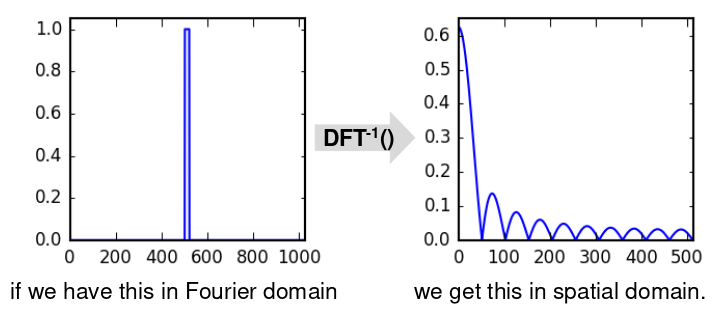
\includegraphics[scale=0.7]{low_pass}
\end{center}
\subsection{Gaussian low pass filter}
\[
G\left(k_{x}, k_{y}\right)=\exp \left[-\left(k_{x}^{2}+k_{y}^{2}\right) / 2 \sigma^{2}\right]
\]
$\sigma$ is the width of the filter at $1/e$. It controls the bandwidth of this filter i.e. the range of frequencies allowed through\\
\\
The Fourier transform of a Gaussian is a Gaussian. Therefore, via convolution theorem, we have the same effect as spatial linear filtering.
\subsection{Butterworth low pass filter}
This is an alternative to the Gaussian\\
\\
\textbf{Operation}: smooth approximation ot the ideal low pass filter to avoid ringing effects
\[
B\left(k_{x}, k_{y}\right)=\frac{1}{1+\left(\frac{\sqrt{k_{k}^{2}+k_{y}^{2}}}{K}\right)^{2 n}}
\]
where n is a user-define positive integer called the order of the filter\\
\\
As n increases, the filter approaches the ideal filter with cut-off value K
\section{Band pass filtering}
\textbf{Operation}: a filter with two frequency thresholds that passes frequencies in a given range
\section{Correlation}
\textbf{Correlation} in image processing is a basic image template matching technique very similar to convolution.\\
\\
They key difference is that masks are not necessarily symmetric\\
\\
Correlation is primarily used to matching, e.g. template matching. The mask represents a template and the response of the mask relates to how well that mask matches the image at a given position, i.e. pixel difference in spatial domain:
\[
I_{output} (i, j)=\sum_{k=-\lfloor N / 2]}^{\lfloor N / 2\rfloor} \sum_{l=-[M / 2]}^{\lfloor M / 2\rfloor}\left\|I_{i n p u t}(i+k, j+l)-m_{k l}\right\|
\]
Applied as per 2D convolution example at each pixel location. Often squared difference is used
\section{Fourier space correlation}
\textbf{Operation}: Find all the regions with certain properties or patterns\\
\\
\textbf{Process} (in Fourier): Transform image and mask into Fourier space and multiply them together. Frequencies in mask are amplified, whilst others attenuated
\section{Deconvolution}
To reverse the effect of a given filter, divide the image by the mask in Fourier space\\
\\
It is the inverse of convolution and is used as basis for image deblurring




\end{document}